\documentclass{isddmaster}
\usepackage[skip=3pt plus1pt]{parskip}
\setlength{\textfloatsep}{12pt plus 2pt minus 4pt}
\setlength{\intextsep}{10pt plus 2pt minus 4pt}
\usepackage{titlesec}
\usepackage{floatrow}
\usepackage{placeins}
\titlespacing*{\subsection}{0pt}{12pt}{4pt}
\onehalfspacing

\begin{document}
	
	\checkyears
	
	\vspace*{5mm}
	
	\setkeys{Gin}{draft=false}
	
	\selectlanguage{french}   
	
	\def\title{Projet de Criblage Virtuel \\[5mm] \normalsize \textit{UE "Chemoinformatics tools for biological therapeutics"}}


	
	\def\spe{Modélisation des macromolécules} 
	% \def\scientificmanager{L. Regad \& M. Baillif}
	\def\author{Anna Perova}
	\def\studentnumber{22519413}
	\def\shorttitle{Rapport Criblage}
	\def\mydate{\today}
	
	\pagenumbering{gobble}
	\Entete
	\medskip
	\begin{abstract}
		{\small \textbf{Résumé:} Ce projet vise à mettre en place et évaluer une procédure de criblage virtuel contre HMG-CoA réductase (HMGCR, UniProt P04035), cible pharmacologique des statines, à partir d'un jeu de 151 composés actifs et 8~324 composés inactifs. Trois approches complémentaires ont été développées et comparées : un criblage \textit{ligand-based} fondé sur la similarité de Tanimoto et de Dice (empreintes MACCS et Morgan) par rapport à un panel de molécules actives de référence ; un criblage \textit{structure-based} par amarrage moléculaire (AutoDock Vina et Smina) sur la structure cristallographique 3CCW ; et un score consensus combinant les deux approches à l'aide de modèles de régression logistique et de forêt aléatoire (\textit{Random Forest}). Les performances ont été évaluées à l'aide de courbes ROC et de courbes d'enrichissement. Le criblage ligand-based, appliqué à la bibliothèque complète, obtient les meilleures performances individuelles (AUC $=93.1\%$ avec les empreintes de Morgan), tandis que le modèle consensus permet d'intégrer l'information structurale sur le sous-échantillon docké.
		
		\textbf{Mots clés:} HMG-CoA réductase ; criblage virtuel ; \textit{ligand-based screening} ; docking moléculaire ; AutoDock Vina ; Smina ; apprentissage automatique ; forêt aléatoire ; courbe d'enrichissement}
	\end{abstract}
	
	\vfill

	%\newpage
	%\tableofcontents
	\newpage
	
	\pagenumbering{arabic}
	\setcounter{page}{1}
	\section{Introduction}
	\textbf{HMG-CoA réductase} (HMGCR), ou 3-hydroxy-3-méthyl-glutaryl-coenzyme A réductase, est une enzyme qui catalyse la transformation du HMG-CoA en L-mévalonate, une étape clé de la voie de biosynthèse du cholestérol et d'autres isoprénoïdes.
	Les inhibiteurs de HMGCR sont principalement utilisés pour traiter la dyslipidémie, qui se traduit par une concentration anormalement élevée (ou, plus rarement, diminuée) de lipides dans le sang. Des taux anormaux de cholestérol sont couramment à l'origine de maladies cardiovasculaires.
	Plus connus sous le nom de statines, les inhibiteurs de HMGCR sont étudiés depuis les années 1970 \cite{endoML236AML236BML236C1976b,endoCompetitiveInhibition3hydroxy3methylglutaryl1976}, et c'est dans les années 1990 que le bénéfice du traitement chez les patients coronariens a été démontré \cite{RandomisedTrialCholesterol}.
	Leur action repose sur l'occupation du site actif de l'enzyme à la place du substrat naturel. % TODO: ajouter ici une référence sur le mécanisme d'action / la structure catalytique de HMGCR (les références [3] et [4] du brouillon original ne portaient pas sur ce point et ont été retirées).
	Malgré leur efficacité, l'utilisation des statines à long terme entraîne des effets secondaires tels que faiblesse musculaire, douleurs nerveuses, surcharge hépatique et fatigue. De plus, certains patients présentent des prédispositions génétiques qui entraînent une intolérance aux statines, d'où l'intérêt de rechercher des structures chimiques alternatives.
	Le développement de pipelines et de modèles prédictifs efficaces pour le criblage virtuel pourrait accélérer le processus de développement pharmaceutique.

	L'objectif de ce projet était d'établir une procédure de criblage virtuel contre une cible bien étudiée et validée pharmacologiquement, HMGCR.
	Cette approche permet de développer et de valider une méthode de criblage virtuel sur des données bien étiquetées, avant de l'appliquer au criblage de structures dont l'activité est inconnue.
	Nous décrivons ici la mise en place d'une procédure permettant d'extraire le nombre maximal de composés actifs parmi les composés les mieux classés, à partir d'un ensemble de 151 composés actifs et 8~324 composés inactifs, en combinant des approches basées sur les ligands, sur la structure, et un score consensus obtenu par régression logistique et forêt aléatoire (\textit{Random Forest}).

	\FloatBarrier
	\section{Préparation des données}
	Les fichiers \lstinline{.smi} contenant les numéros d'identification ChEMBL et les structures au format SMILES ont été fournis pour ce projet \footnote{\href{https://owncloud.rpbs.univ-paris-diderot.fr/owncloud/index.php/s/J3z2UQGxRhSr5YY}{Lien pour les données}}. Ils contiennent 151 composés actifs et 8~324 composés inactifs.
	Le traitement des données et l'analyse ont été effectués dans un notebook Jupyter en Python \footnote{\href{https://github.com/annhater/My-Vault}{Données pour l'ensemble du projet sur GitHub}}.
	Une vérification de l'activité de ces composés a été réalisée à l'aide de la métrique pIC50 (pIC50 $\geq 6.5$, soit IC50 $\leq$ 316~nM environ). % TODO: confirmer que ce seuil correspond exactement à celui utilisé dans le notebook (le brouillon original indiquait « IC50 $\geq$ 6.5 nM », ce qui mélangeait IC50 et pIC50 ; à vérifier).
	L'absence de duplicats dans le jeu de données a ensuite été confirmée, et les structures SMILES ont été préparées pour les traitements suivants en supprimant les sels à l'aide du package \lstinline{RDKit}.
	Vingt structures choisies aléatoirement ont été retenues comme structures actives de référence pour le calcul du taux de similarité par la suite (Figure~\ref{fig:ref_set}). Ainsi, pour l'étape de criblage ligand-based, 280 molécules actives et 8~324 molécules inactives ont été conservées.

	\begin{figure}[!ht]
		\centering
		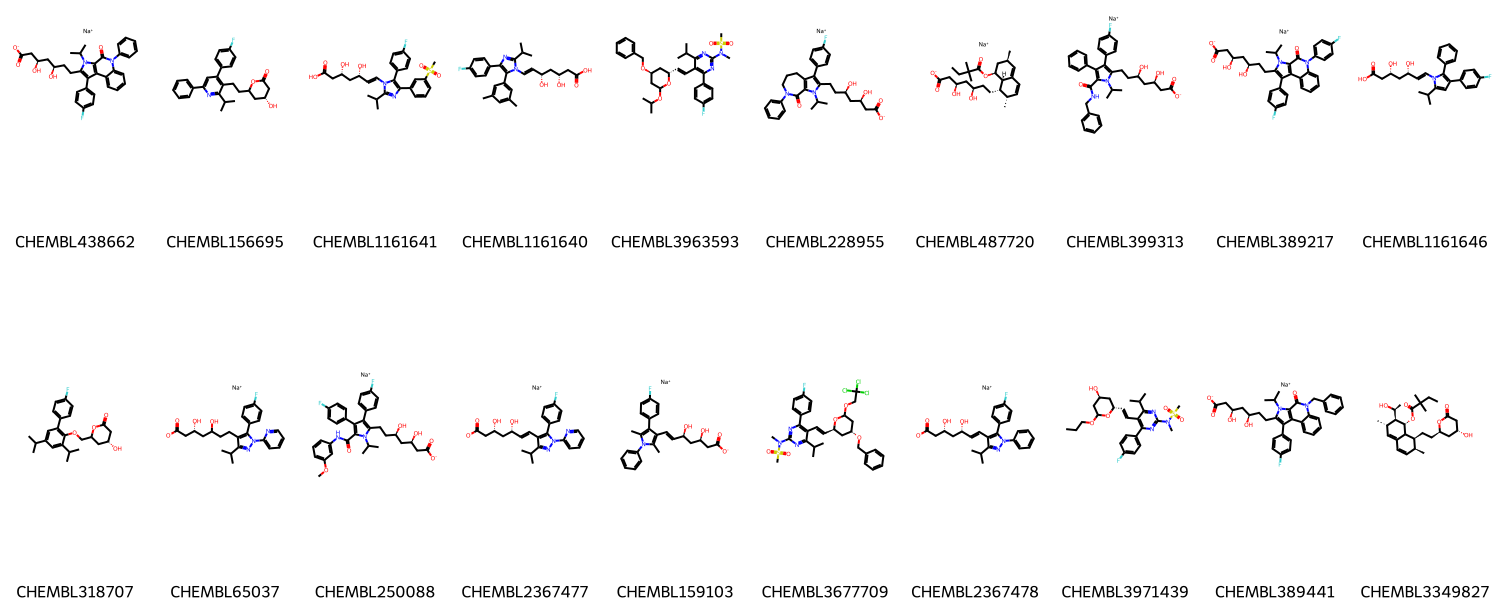
\includegraphics[width=\textwidth]{Figures/ref_set.png}
		\caption{Dataset de molécules actives choisies comme référence pour le criblage ligand-based.}
		\label{fig:ref_set}
	\end{figure}

	\FloatBarrier
	\section{Ligand-based screening}
	
	\begin{wrapfigure}[14]{r}{0.5\textwidth}
		\vspace{-10mm}
        \begin{center}
			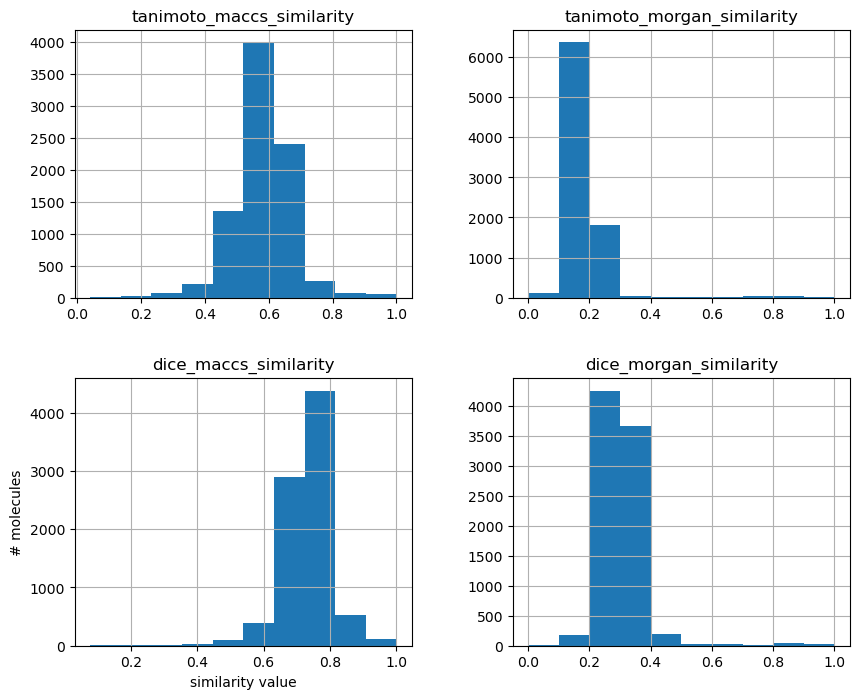
\includegraphics[width=\textwidth]{Figures/sim_hist.png}
			\caption{Distribution des scores de similarité (Tanimoto et Dice, empreintes MACCS et Morgan) entre les molécules de la librairie et les 20 structures actives de référence.}
		\label{fig:hist}
		\end{center}
	\end{wrapfigure}
	Les empreintes de Morgan (2048 bits, rayon 2) et MACCS (167 bits) ont été calculées pour l'ensemble des molécules.
	À partir de ces empreintes, les taux de similarité ont été obtenus avec deux coefficients : Tanimoto et Dice (Figure~\ref{fig:hist}).
	En analysant les distributions de ces scores, on observe que les clés MACCS produisent des taux de similarité moins élevés -- ce qui est cohérent avec la sensibilité plus fine de cet algorithme, qui capture l'environnement atomique de façon plus détaillée.
	Le coefficient de Dice, quant à lui, tend à produire des valeurs plus élevées, du fait de son mode de calcul qui accorde davantage de poids à l'intersection entre les deux empreintes. Ne souhaitant pas trop privilégier les similarités entre molécules actives et inactives tout en capturant l'environnement chimique le plus précis possible, le score \lstinline{tanimoto_morgan_similarity} a été retenu pour la suite de l'analyse.

	\begin{wrapfigure}[10]{r}{0.4\textwidth}
		\vspace{-5mm}
        \begin{center}
			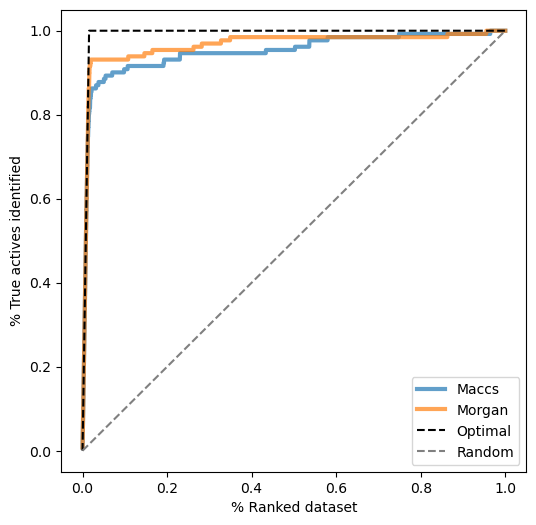
\includegraphics[width=0.8\linewidth]{Figures/roc_ligand.png}
			\caption{Courbes d'enrichissement pour les deux métriques : score de Tanimoto avec les empreintes de Morgan (orange, AUC $=93.1\%$) ou de MACCS (bleu, AUC $=87.8\%$).}
		\label{fig:roc-ligand}
		\end{center}
	\end{wrapfigure}
	Par la suite, afin d'évaluer et de valider les résultats du criblage virtuel basé sur les ligands, des courbes d'enrichissement ont été construites (Figure~\ref{fig:roc-ligand}). Elles représentent la proportion de molécules actives détectées parmi les x\% les mieux classées, par rapport à la proportion de molécules actives dans l'ensemble du jeu de données.
	Les résultats démontrent que la méthode de criblage virtuel utilisant les empreintes de Morgan identifie avec succès une proportion plus élevée de molécules réellement actives dès le début de la liste classée, comparativement à une sélection aléatoire . En utilisant les empreintes de MACCS les résultats sont comparables.
	On peut conclure que le criblage ligand-based fondé sur la similarité de Tanimoto avec les empreintes de Morgan constitue une méthode rapide et efficace pour prioriser les composés sur l'ensemble de la bibliothèque, en amont de l'étape plus coûteuse de docking moléculaire.

	\FloatBarrier
	\section{Structure-based screening (docking)}
	\begin{wrapfigure}[18]{r}{0.45\textwidth}
		\begin{center}
			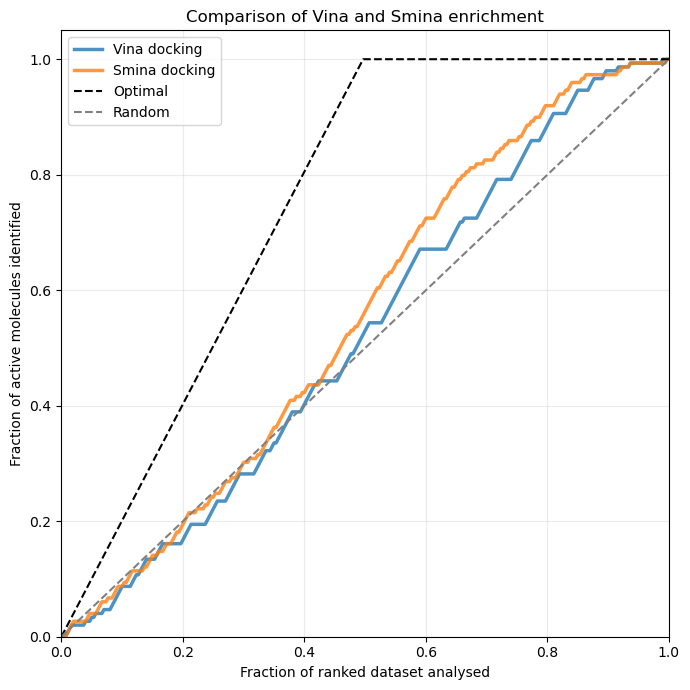
\includegraphics[width=0.8\linewidth]{Figures/vina-smina.png}
			\caption{Courbes d'enrichissement pour les deux outils de docking : Smina (orange, AUC $=40\%$) et Vina (bleu, AUC $=$ \textit{à compléter}). \small\textit{Note~: une AUC inférieure à 50\% correspond à une performance pire que l'aléatoire ; cette valeur mérite d'être revérifiée avant soumission (possible inversion du sens du score, un score de docking plus négatif correspondant à une meilleure affinité).}}
		\label{fig:vina-smina}
		\end{center}
	\end{wrapfigure}
	L'étude de la structure des ligands constitue une bonne approche d'analyse préliminaire ; néanmoins, il est également important de comprendre la façon dont le ligand interagit avec la cible/le récepteur. Pour cela, des méthodes d'amarrage moléculaire (\textit{docking}) sont appliquées.
	La structure utilisée pour l'amarrage est celle de l'entrée 3CCW de la PDB \footnote{\href{https://www.rcsb.org/structure/3CCW}{Entrée web sur PDB}}, produit de la co-cristallisation de HMGCR avec 4HI (molécule apparentée aux statines \footnote{\href{https://www.ebi.ac.uk/chembl/explore/compound/CHEMBL488636}{Entrée ChEMBL}}), obtenue par diffraction aux rayons X à une résolution de 2.1\AA\ (Figure~\ref{fig:3ccw}).\\
	Afin de préparer la structure pour l'amarrage, l'eau a été éliminée, les charges assignées, et le fichier converti du format \lstinline{.mol2} au format \lstinline{.pdbqt} à l'aide de l'outil OpenBabel \footnote{\href{https://openbabel.org/index.html}{Site web de OpenBabel}}.
	Le centre de la boîte de docking a été déterminé à partir du centre du ligand 4HI dans la structure d'origine (x~: 4.76321, y~: 31.71096, z~: 6.64880), avec une taille de boîte de $30\times30\times30$~\AA.


	\begin{figure}[!ht]
		\centering
		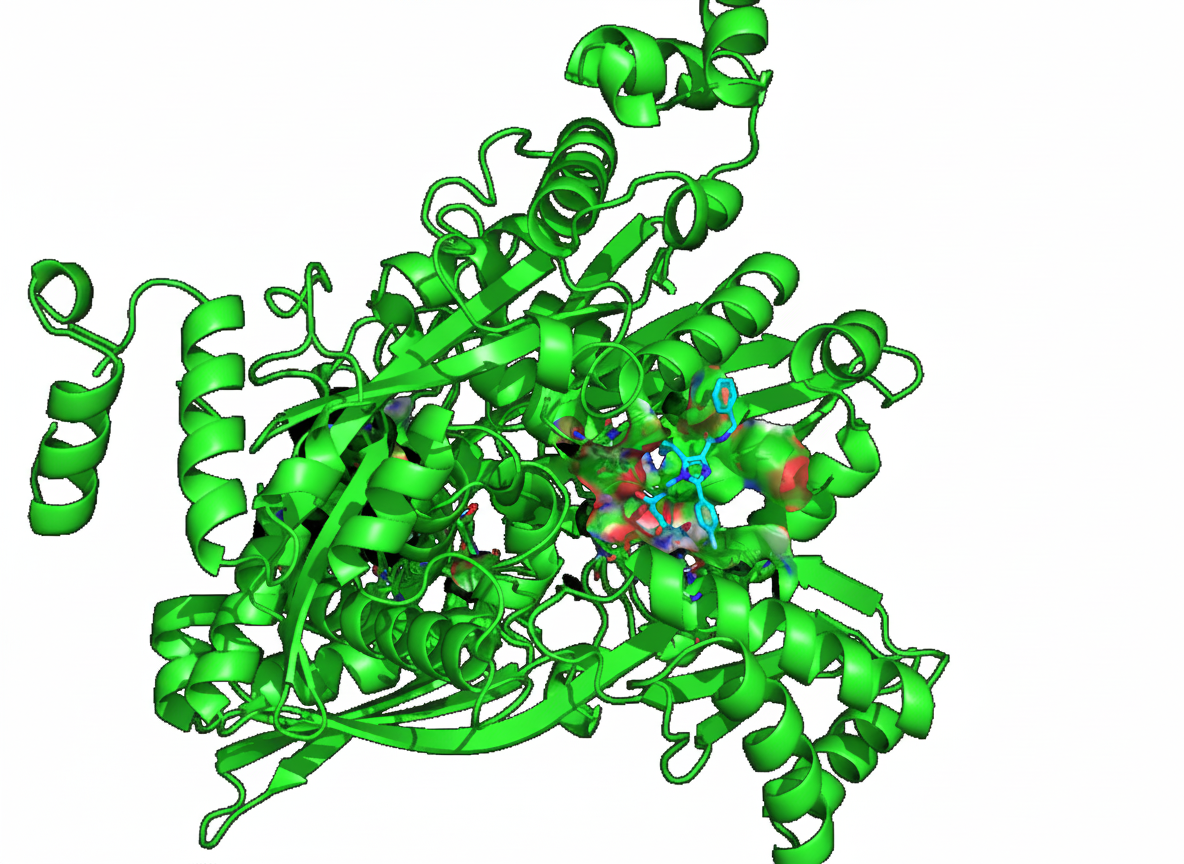
\includegraphics[width=0.6\textwidth]{Figures/3CCW.png}
		\caption{Représentation 3D de HMGCR (vert) avec le ligand 4HI (cyan) dans la poche d'interaction, visualisée avec PyMOL. PDB : 3CCW.}
		\label{fig:3ccw}
	\end{figure}

	Pour les 151 ligands actifs et 151 inactifs (choisis aléatoirement), une structure \lstinline{.pdbqt} a été générée avec OpenBabel (seules 149 structures actives ont pu être converties, la génération 3D ayant échoué pour CHEMBL3704922 et CHEMBL3704923). Le choix de ne retenir que 151 molécules inactives sur les 8~324 composés d'origine s'explique principalement par des contraintes de temps (le docking de l'ensemble de la bibliothèque inactive aurait nécessité environ 5 jours de calcul). Ce sous-échantillonnage permet non seulement de comparer les résultats de deux outils de docking, mais aussi d'obtenir un jeu de données équilibré par rapport à la portion de molécules actives (un déséquilibre pouvant introduire un biais dans les modèles d'apprentissage développés par la suite).
	Deux logiciels de docking ont été utilisés : AutoDock Vina et Smina, une version dérivée d'AutoDock Vina proposant une fonction de score améliorée et une minimisation d'énergie plus performante.
	Après le docking, le score d'énergie potentielle de la pose la plus favorable énergétiquement a été extrait pour chaque composé, ainsi que les données d'enrichissement correspondantes (Figure~\ref{fig:vina-smina}).
	Les courbes d'enrichissement montrent que Smina obtient de meilleures performances qu'AutoDock Vina ; les deux outils présentent cependant une différence limitée par rapport à la courbe d'enrichissement aléatoire (obtenue en sélectionnant les composés de manière totalement aléatoire).
	Ceci est globalement cohérent avec la littérature, qui indique qu'un score de docking brut tel que celui de Vina est souvent moins performant qu'une approche combinant plusieurs sources d'information \cite{Confidence}. % TODO: vérifier que cette référence appuie bien cette affirmation précise.

	Ainsi, un modèle prédictif (régression logistique, puis forêt aléatoire) a ensuite été mis en place, combinant les résultats du criblage ligand-based et structure-based.
	
	\FloatBarrier
	\section{Méthode consensus (apprentissage automatique)}

	Pour entraîner les modèles de régression logistique et de forêt aléatoire (\textit{Random Forest}), deux descripteurs ont été retenus : le score de similarité (Tanimoto sur empreintes Morgan) et le score d'amarrage (Smina). Lors du développement du modèle, un sur-apprentissage a été observé, indiqué par des métriques de rappel et d'exactitude proches de 1.
	Afin d'éviter ce type de sur-apprentissage, une attention particulière a été portée à ce que les structures chimiquement trop proches ne soient pas réparties entre les jeux d'entraînement et de test, mais restent regroupées dans un seul des deux jeux.
	Pour cela, l'approche des squelettes de Bemis-Murcko, introduite en 1996 et implémentée dans RDKit, a été appliquée \cite{bemisPropertiesKnownDrugs1996,huLessonsLearnedMolecular2011}.

	En analysant les performances des deux modèles consensus (Figure~\ref{fig:all}), on observe que la forêt aléatoire est nettement plus performante que la régression logistique. Ce résultat est attendu, la forêt aléatoire étant mieux adaptée à la gestion de relations non linéaires ainsi qu'à la multicolinéarité présente entre les deux descripteurs. 
	Néanmoins, en comparant avec les autres tests réalisés, on observe que, sur ce sous-ensemble de ligands, l'analyse sans intégrer les données issues du docking donne des performances plus élevées. Cela peut indiquer que, pour ce sous-ensemble particulier, les résultats de docking apportent une complexité additionnelle qui réduit la performance du modèle.
	Cela étant dit, il n'est pas possible d'affirmer que cette observation se généraliserait à un autre sous-ensemble, ou à des données totalement nouvelles et non étiquetées. Il est donc préférable de conserver le modèle consensus, qui combine l'information provenant à la fois des ligands et du récepteur.

	\begin{figure}[!ht]
		\centering
		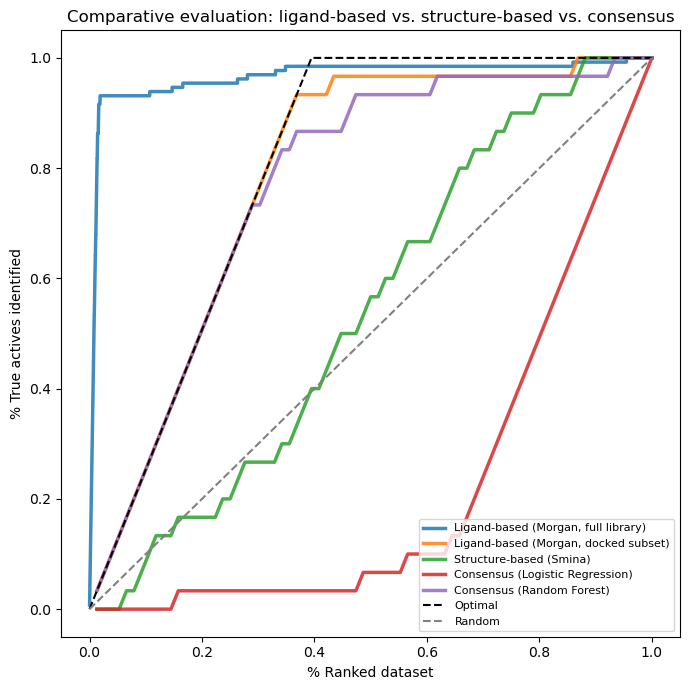
\includegraphics[width=0.7\textwidth]{Figures/comparative_evaluation.png}
		\caption{Comparaison des courbes d'enrichissement pour le criblage ligand-based (bibliothèque complète en bleu et sous-échantillon docké en orange), le criblage structure-based (Smina) en vert et les modèles consensus (régression logistique en rouge et forêt aléatoire en violet), évalués sur le jeu de test (\textit{scaffold split}).}
		\label{fig:all}
	\end{figure}
	
	\FloatBarrier
	\section{Discussion et conclusion}
	Ce projet de criblage virtuel a permis de mettre en place et de comparer trois approches complémentaires -- ligand-based, structure-based et consensus -- pour la priorisation de composés actifs contre HMGCR.
	La méthode basée sur les ligands est capable d'analyser la bibliothèque complète avec un bon niveau de performance (AUC $=93.1\%$ avec les empreintes de Morgan). Les résultats basés sur l'analyse de structure et sur le méthode consensus sont, quant à eux, limités à un sous-échantillon représentatif en raison du coût de calcul de l'amarrage moléculaire. Néanmoins ces informations structurales apportent des caractéristiques indispensables qui pourraient se révéler utiles lors de l'application de ce modèle à un jeu de données réel et non étiqueté.
	Malgré la présence, dans le jeu d'inactifs, de composés structurellement proches des actifs mais expérimentalement confirmés inactifs (\textit{decoys}), notre méthode a permis de bien distinguer les molécules actives : les dix molécules présentant les scores de similarité Tanimoto-Morgan les plus élevés sont exclusivement des composés actifs (Figure~\ref{fig:top-10}).

	Plusieurs limites de ce travail doivent être soulignées. Premièrement, l'évaluation structure-based et consensus repose sur un sous-échantillon de 300 molécules et ne couvre donc pas l'ensemble de la bibliothèque d'inactifs. Deuxièmement, la procédure n'a pas été validée sur un jeu de données externe indépendant.
	En perspective, il serait donc intéressant de tester ce protocole contre un \textit{benchmark} public externe (DUD-E ou DEKOIS), afin de confirmer sa capacité de généralisation sur des données nouvelles. Il serait également pertinent d'étendre le docking à un plus grand nombre de composés inactifs, sous réserve de ressources de calcul suffisantes, et d'explorer des fonctions de \textit{rescoring} basées sur l'apprentissage automatique (par exemple RF-Score-VS ou CNN-Score), comme proposé dans l'article de référence fourni pour ce projet \cite{tran-nguyenPracticalGuideMachinelearning2023}.

	\begin{figure}[!ht]
		\centering
		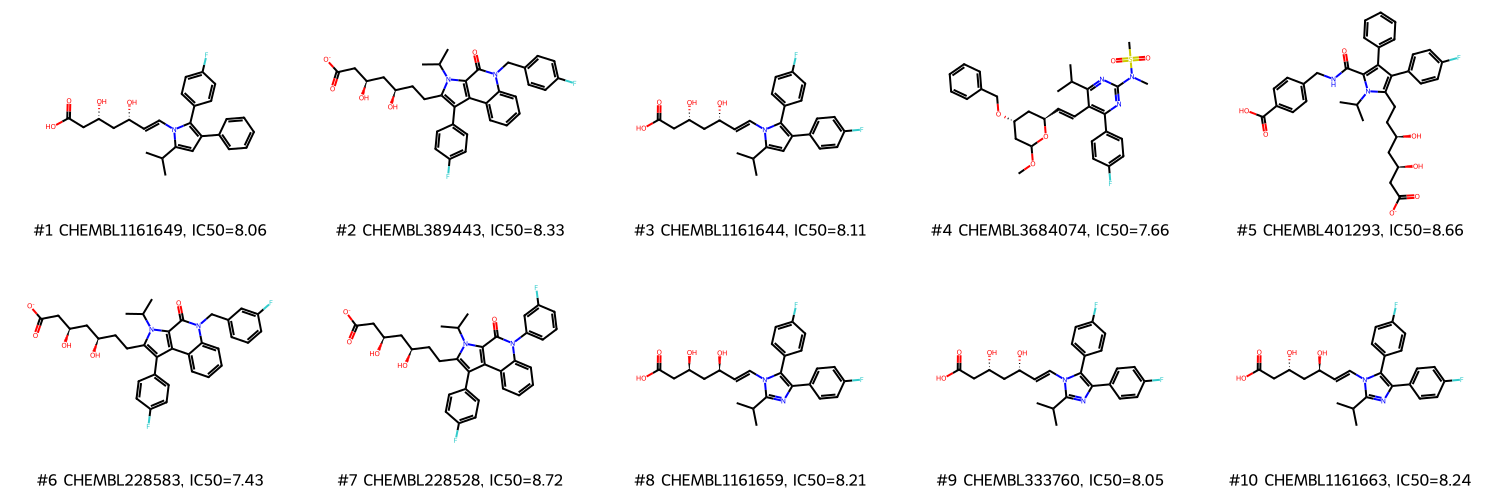
\includegraphics[width=\textwidth]{Figures/top-10.png}
		\caption{Les dix molécules avec les scores de similarité Tanimoto-Morgan les plus élevés contre les actives de référence. Toutes ces molécules font partie du jeu de données de molécules actives d'origine.}
		\label{fig:top-10}
	\end{figure}
	\FloatBarrier
	\addcontentsline{toc}{section}{Références}
	\bibliographystyle{unsrt} 
	\bibliography{masterBib} 
	\cleardoublepage
	
\end{document}